\documentclass[
  11pt,
  letterpaper,
   addpoints,
  answers
  ]{exam}

% Carga el preámbulo localizado en la carpeta superior
\NeedsTeXFormat{LaTeX2e}[2023/04/30]

% Provide the name of your page, the date it was last updated, and a comment about what it's used for
\ProvidesPackage{../exercise-preamble}[2023/04/30 Prof. Cassanelli custom LaTeX style]

% \usepackage{printlen}
% \uselengthunit{in}\printlength{\textwidth}

% PACKAGES
\usepackage[dvipsnames]{xcolor}

\usepackage{graphicx}
\graphicspath{{../figures}}
\usepackage{amsmath,amsthm,amssymb,mathtools,mathrsfs}
\usepackage{commath}
\usepackage{upgreek}
\usepackage{cancel}
\usepackage{enumerate}
\usepackage[font=small]{caption}
\usepackage[normalem]{ulem}
\usepackage{steinmetz}

\usepackage[left=1.5cm, right=1.5cm, top=1cm]{geometry}

% REFERENCES AND OTHERS
\usepackage{../aas_macros}
\usepackage{natbib}
\bibpunct{(}{)}{;}{a}{}{,}

\usepackage{tikz}
\usepackage{tikz-3dplot}
\usepackage{circuitikz}
\usepackage{pgfplots}
\pgfplotsset{compat=1.15}
\usepgfplotslibrary{smithchart}
\usetikzlibrary{
  decorations.pathmorphing,
  decorations.markings,
  calc,
  patterns,
  decorations,
  angles,
  quotes,
  ext.topaths.arcthrough,
  shapes
  }

\usepackage{siunitx}
\sisetup{
    range-phrase=\text{--},
    range-units=single,
    separate-uncertainty=true,
    print-unity-mantissa=false
    }
\DeclareSIUnit{\gauss}{G}
\DeclareSIUnit{\jansky}{Jy}

\newcommand{\iu}{\mathrm{i}\mkern1mu}
\newcommand{\ju}{\mathrm{j}\mkern1mu}
\newcommand{\euler}{\mathrm{e}}
\newcommand{\exponential}[1]{\mathrm{exp}\left[#1\right]}
\newcommand{\uvec}[1]{\widehat{\mathbf{#1}}}
\newcommand{\uvecs}[1]{\boldsymbol{\widehat{#1}}}
\newcommand{\bvec}[1]{\boldsymbol{\mathcal{#1}}}

\usepackage{hyperref}
\hypersetup{
    % bookmarks=true,
    unicode=true,
    pdftoolbar=true,
    pdfmenubar=true,
    pdffitwindow=false,
    pdfstartview={FitH},
    pdftitle={EL3103},
    pdfauthor={Tomas Cassanelli},
    pdfcreator={Tomas Cassanelli},
    pdfnewwindow=true,
    colorlinks=true,
    linkcolor=Violet,
    citecolor=Violet,
    urlcolor=Violet
    }

% Exam document class
\renewcommand{\figurename}{Figura}
\renewcommand{\tablename}{Cuadro}
\pagestyle{empty}

\usepackage[spanish]{cleveref}

\crefname{question}{\protect{pregunta}}{\protect{preguntas}}
\Crefname{question}{\protect{Pregunta}}{\protect{Preguntas}}
\creflabelformat{question}{#2{#1}#3}

\renewcommand{\solutiontitle}{\noindent\textbf{Solución:}\par\noindent}
\bracketedpoints
\pointname{~puntos}

\endinput

% Paquetes locales
\usepackage{float}
\usepackage{booktabs} % para \toprule, \midrule, \bottomrule
\usepackage{xcolor} % para colores
\usepackage{bm} % para negrita en símbolos matemáticos

% Macros locales
\newcommand{\Rel}{\mathfrak{R}} % símbolo para la reluctancia

\begin{document}

% Numeración de página
\pagestyle{plain}
\pagenumbering{arabic}

\noindent
\begin{minipage}{0.47\textwidth}
\includegraphics[width=\textwidth]{../fcfm_die}
\end{minipage}
\begin{minipage}{0.53\textwidth}
\begin{center} 
\large\textbf{Análisis de Sistemas Dinámicos y Estimación} (EL3204-1) \\
\large\textbf{Clase auxiliar 7} \\
\normalsize Prof.~ Marcos Orchard - Sebastián Espinosa.\\
\normalsize Prof.~Aux.~Erik Sáez
\end{center}
\end{minipage}

\vspace{0.5cm}
\noindent
\vspace{.85cm}
%----------------------------
\section{Resumen}

\subsubsection*{Variables Aleatorias}

Una \textbf{variable aleatoria} $X$ es una función que asigna un número real a cada resultado de un experimento aleatorio: $X : \Omega \longrightarrow \mathbb{R}$. En la práctica, trabajamos con las distribuciones de estas variables.\\

Las variables continuas tienen una \textbf{función de densidad de probabilidad} $f(x)$ que describe qué tan ``densa'' es la probabilidad alrededor de cada punto. No da probabilidades directas, sino que las probabilidades se calculan integrando: $\mathbb{P}(a \leq X \leq b) = \int_a^b f(x) \, dx$. Debe cumplir $f(x) \geq 0$ y $\int_{-\infty}^{\infty} f(x) \, dx = 1$.\\

Las variables discretas tienen una \textbf{función de probabilidad de masa} $p(x)$ que da directamente la probabilidad de cada valor específico. Debe cumplir $p(x) \geq 0$ y $\sum_{x} p(x) = 1$. Las probabilidades se calculan sumando: $\mathbb{P}(X \in A) = \sum_{x \in A} p(x)$.

\subsubsection*{Distribuciones Importantes}

\textbf{Distribución Uniforme} $X \sim U(a,b)$: Todos los valores en $[a,b]$ son igualmente probables.
\begin{equation}
f(x) = \begin{cases}
\frac{1}{b-a} & \text{si } x \in [a,b] \\
0 & \text{en otro caso}
\end{cases}
\end{equation}

\textbf{Distribución Exponencial} $X \sim \text{Exp}(\lambda)$: Modela tiempos de espera entre eventos. 
\begin{equation}
f(x) = \begin{cases}
\lambda e^{-\lambda x} & \text{si } x \geq 0 \\
0 & \text{en otro caso}
\end{cases}
\end{equation}

\textbf{Distribución Normal} $X \sim \mathcal{N}(\mu, \sigma^2)$: La distribución más importante. Curva en forma de campana.
\begin{equation}
f(x) = \frac{1}{\sqrt{2\pi}\sigma} \exp\left(-\frac{(x-\mu)^2}{2\sigma^2}\right)
\end{equation}
Propiedad clave: cualquier combinación lineal de variables normales independientes también es normal.

\textbf{Distribución Poisson} $X \sim \text{Poisson}(\lambda)$: Modela el número de eventos raros en un intervalo fijo.
\begin{equation}
p(x) = \begin{cases}
\frac{e^{-\lambda}\lambda^x}{x!} & \text{si } x \in \{0, 1, 2, \ldots\} \\
0 & \text{en otro caso}
\end{cases}
\end{equation}

\subsubsection*{Vectores Aleatorios}

Un \textbf{vector aleatorio} $\mathbf{X} = (X_1, X_2, \ldots, X_n)$ agrupa múltiples variables aleatorias. Su \textbf{función de densidad conjunta} describe el comportamiento conjunto:
\begin{equation}
f_{\mathbf{X}}(\mathbf{x}) = f_{X_1,X_2,\ldots,X_n}(x_1, x_2, \ldots, x_n)
\end{equation}

Para variables \textbf{independientes e idénticamente distribuidas (i.i.d.)}:
\begin{equation}
f_{\mathbf{X}}(\mathbf{x}) = \prod_{i=1}^n f_{X_i}(x_i)
\end{equation}

\subsubsection*{Momentos Estadísticos}

Los \textbf{momentos} caracterizan las propiedades de una distribución:

\textbf{Esperanza} (valor promedio esperado):
\begin{align}
\mathbb{E}[X] = \begin{cases}
\int_{-\infty}^{\infty} x \cdot f(x) \, dx & \text{si } X \text{ es continua} \\
\sum_x x \cdot p(x) & \text{si } X \text{ es discreta}
\end{cases}
\end{align}

\textbf{Varianza} (medida de dispersión):
\begin{equation}
\text{Var}(X) = \mathbb{E}[X^2] - (\mathbb{E}[X])^2
\end{equation}

\textbf{Covarianza} (dependencia lineal entre dos variables):
\begin{equation}
\text{Cov}(X,Y) = \mathbb{E}[XY] - \mathbb{E}[X]\mathbb{E}[Y]
\end{equation}

Para la distribución normal $X \sim \mathcal{N}(\mu, \sigma^2)$: $\mu = \mathbb{E}[X]$ y $\sigma^2 = \text{Var}(X)$.
\newpage
%----------------------------
\begin{questions}
  \question Responda las siguientes preguntas:
  \begin{enumerate}
    \item Sea $X$ una variable aleatoria discreta tal que $X \sim \text{poisson}(\lambda)$, obtenga su esperanza y su varianza.
    
    \item Sean $X_1, X_2, \ldots, X_n$ variables aleatorias continuas i.i.d tal que cada una distribuye $\mathcal{N}(\mu, \sigma^2)$. Obtenga su distribución conjunta.
    
    \item Sean $X_1, X_2, \ldots, X_n$ variables aleatorias continuas i.i.d tal que cada una distribuye $\mathcal{N}(\mu, \sigma^2)$. Obtenga la distribución de $Y = \sum_{i=1}^{n} \frac{X_i - \mu}{\sqrt{n}\sigma}$.
  \end{enumerate}
%----------------------------
\begin{solution}
  \subsection*{Resolución 1.1}
  
  Para una variable aleatoria $X$ que sigue una distribución de Poisson con parámetro $\lambda$, recordemos que su función de probabilidad de masa está dada por $P(X = x) = \frac{e^{-\lambda} \lambda^x}{x!}$ para $x = 0, 1, 2, \ldots$
  
  Para obtener la esperanza, aplicamos la definición correspondiente a variables aleatorias discretas. Calculamos $\mathbb{E}[X] = \sum_{x=0}^{\infty} x \cdot P(X = x) = \sum_{x=0}^{\infty} x \cdot \frac{e^{-\lambda} \lambda^x}{x!}$. Observamos que el término con $x = 0$ es igual a cero, por lo que podemos reescribir la suma como:
  \begin{align}
  \mathbb{E}[X] &= \sum_{x=1}^{\infty} x \cdot \frac{e^{-\lambda} \lambda^x}{x!} = \sum_{x=1}^{\infty} \frac{e^{-\lambda} \lambda^x}{(x-1)!} = e^{-\lambda} \lambda \sum_{x=1}^{\infty} \frac{\lambda^{x-1}}{(x-1)!}
  \end{align}
  
  Al realizar el cambio de variable $u = x - 1$, obtenemos:
  \begin{equation}
  \mathbb{E}[X] = e^{-\lambda} \lambda \sum_{u=0}^{\infty} \frac{\lambda^u}{u!}
  \end{equation}
  
  La sumatoria que aparece corresponde exactamente a la serie de Taylor de la función exponencial $e^x = \sum_{n=0}^{\infty} \frac{x^n}{n!}$. Por tanto, $\sum_{u=0}^{\infty} \frac{\lambda^u}{u!} = e^{\lambda}$, lo que nos da:
  \begin{equation}
  \mathbb{E}[X] = e^{-\lambda} \cdot \lambda \cdot e^{\lambda} = \lambda
  \end{equation}
  
  Para calcular la varianza, utilizamos la fórmula $\text{Var}(X) = \mathbb{E}[X^2] - [\mathbb{E}[X]]^2$ y necesitamos determinar $\mathbb{E}[X^2]$. Siguiendo un procedimiento similar al anterior:
  \begin{align}
  \mathbb{E}[X^2] &= \sum_{x=0}^{\infty} x^2 \cdot \frac{e^{-\lambda} \lambda^x}{x!} = \sum_{x=1}^{\infty} x^2 \cdot \frac{e^{-\lambda} \lambda^x}{x!}\\
  &= \sum_{x=1}^{\infty} x \cdot \frac{e^{-\lambda} \lambda^x}{(x-1)!} = e^{-\lambda} \lambda \sum_{x=1}^{\infty} x \cdot \frac{\lambda^{x-1}}{(x-1)!}
  \end{align}
  
  Con el cambio de variable $u = x - 1$ (de modo que $x = u + 1$), ademas recordemos que $\sum_{u=0}^{\infty} \frac{\lambda^u}{u!} = e^{\lambda}$ y $\sum_{u=0}^{\infty} u \cdot \frac{\lambda^u}{u!} = \lambda e^{\lambda}$, tenemos:
  \begin{align}
  \mathbb{E}[X^2] &= e^{-\lambda} \lambda \sum_{u=0}^{\infty} (u+1) \cdot \frac{\lambda^u}{u!}\\
  &= e^{-\lambda} \lambda \left[ \sum_{u=0}^{\infty} u \cdot \frac{\lambda^u}{u!} + \sum_{u=0}^{\infty} \frac{\lambda^u}{u!} \right]\\
  &= e^{-\lambda} \lambda \left[ \lambda e^{\lambda} + e^{\lambda} \right] = \lambda^2 + \lambda
  \end{align}
  
  Finalmente, la varianza resulta ser:
  \begin{equation}
  \text{Var}(X) = \mathbb{E}[X^2] - [\mathbb{E}[X]]^2 = (\lambda^2 + \lambda) - \lambda^2 = \lambda
  \end{equation}
  
  Concluimos que para una variable aleatoria $X \sim \text{Poisson}(\lambda)$, tanto su esperanza como su varianza son iguales al parámetro $\lambda$.

  \subsection*{Resolución 1.2}
  
  Necesitamos encontrar la función de densidad conjunta de $n$ variables aleatorias $X_1, X_2, \ldots, X_n$ que son independientes e idénticamente distribuidas con distribución $\mathcal{N}(\mu, \sigma^2)$.
  
  Cuando las variables aleatorias son independientes, una propiedad fundamental nos dice que la función de densidad conjunta es simplemente el producto de las funciones de densidad marginales. Es decir:
  \begin{equation}
  f_{X_1,X_2,\ldots,X_n}(x_1, x_2, \ldots, x_n) = \prod_{i=1}^{n} f_{X_i}(x_i)
  \end{equation}
  
  Sabemos que cada variable aleatoria individual $X_i \sim \mathcal{N}(\mu, \sigma^2)$ tiene función de densidad:
  \begin{equation}
  f_{X_i}(x_i) = \frac{1}{\sqrt{2\pi} \sigma} \exp\left(-\frac{(x_i-\mu)^2}{2\sigma^2}\right)
  \end{equation}
  
  Al aplicar la propiedad de independencia y multiplicar todas las densidades marginales:
  \begin{align}
  f_{X_1,X_2,\ldots,X_n}(x_1, \ldots, x_n) &= \prod_{i=1}^{n} \frac{1}{\sqrt{2\pi} \sigma} \exp\left(-\frac{(x_i-\mu)^2}{2\sigma^2}\right)\\
  &= \frac{1}{(\sqrt{2\pi} \sigma)^n} \prod_{i=1}^{n} \exp\left(-\frac{(x_i-\mu)^2}{2\sigma^2}\right)\\
  &= \frac{1}{(2\pi)^{n/2} \sigma^n} \exp\left(-\frac{1}{2\sigma^2} \sum_{i=1}^{n} (x_i - \mu)^2\right)
  \end{align}
  
  Por tanto, la función de densidad conjunta está dada por:
  \begin{equation}
  f_{X_1,X_2,\ldots,X_n}(x_1, \ldots, x_n) = \frac{1}{(2\pi)^{n/2} \sigma^n} \exp\left(-\frac{1}{2\sigma^2} \sum_{i=1}^{n} (x_i - \mu)^2\right)
  \end{equation}
  

  
  Esta expresión corresponde a una \textbf{distribución normal multivariada} (o gaussiana multivariada), que generalizamos como $\mathbf{X} = (X_1, \ldots, X_n) \sim \mathcal{N}(\boldsymbol{\mu}, \boldsymbol{\Sigma})$, donde:
  
  \begin{itemize}
  \item \textbf{Vector de medias:} $\boldsymbol{\mu} = (\mu, \mu, \ldots, \mu)^T \in \mathbb{R}^n$
  
  Cada componente del vector aleatorio tiene la misma media $\mu$, es decir, $\mathbb{E}[X_i] = \mu$ para todo $i = 1, \ldots, n$.
  
  \item \textbf{Matriz de covarianza:} $\boldsymbol{\Sigma} = \sigma^2 I_n$, donde $I_n$ es la matriz identidad de orden $n$:
  \begin{equation}
  \boldsymbol{\Sigma} = \sigma^2 \begin{pmatrix}
  1 & 0 & \cdots & 0 \\
  0 & 1 & \cdots & 0 \\
  \vdots & \vdots & \ddots & \vdots \\
  0 & 0 & \cdots & 1
  \end{pmatrix} = \begin{pmatrix}
  \sigma^2 & 0 & \cdots & 0 \\
  0 & \sigma^2 & \cdots & 0 \\
  \vdots & \vdots & \ddots & \vdots \\
  0 & 0 & \cdots & \sigma^2
  \end{pmatrix}
  \end{equation}
  
  Los elementos de la diagonal principal son $\text{Var}(X_i) = \sigma^2$ para todo $i$, mientras que los elementos fuera de la diagonal son $\text{Cov}(X_i, X_j) = 0$ para $i \neq j$.
  
  \item \textbf{Independencia:} La forma diagonal de $\boldsymbol{\Sigma}$ (con ceros fuera de la diagonal) refleja precisamente que las variables son independientes. En general, para variables normales, covarianza cero implica independencia estadística. Por tanto:
  \begin{equation}
  \text{Cov}(X_i, X_j) = 0 \text{ para } i \neq j \quad \Longleftrightarrow \quad X_i \text{ y } X_j \text{ son independientes}
  \end{equation}
  \end{itemize}
  
  En resumen, podemos escribir que el vector aleatorio $\mathbf{X} = (X_1, \ldots, X_n) \sim \mathcal{N}(\boldsymbol{\mu}, \sigma^2 I_n)$, donde cada variable tiene la misma media $\mu$ y varianza $\sigma^2$, y todas son mutuamente independientes.

  \subsection*{Resolución 1.3}
  
  Se nos pide encontrar la distribución de $Y = \sum_{i=1}^{n} \frac{X_i - \mu}{\sqrt{n}\sigma}$, donde $X_1, X_2, \ldots, X_n$ son variables aleatorias i.i.d. con distribución $\mathcal{N}(\mu, \sigma^2)$.
  
  Como la variable $Y$ es una combinación lineal de variables aleatorias normales independientes, también distribuirá normal (propiedad vista en el recordatorio). Con ello, calculamos la esperanza y su varianza para tener así sus parámetros. Para la esperanza, se tiene:
  \begin{align}
  \mathbb{E}[Y] &= \mathbb{E}\left[\sum_{i=1}^{n} \frac{X_i - \mu}{\sqrt{n}\sigma}\right] = \frac{1}{\sqrt{n}\sigma} \mathbb{E}\left[\sum_{i=1}^{n} (X_i - \mu)\right]\\
  &= \frac{1}{\sqrt{n}\sigma} \left[\sum_{i=1}^{n} \mathbb{E}[X_i - \mu]\right] = \frac{1}{\sqrt{n}\sigma} \left[\sum_{i=1}^{n} (\mathbb{E}[X_i] - \mu)\right]\\
  &= \frac{1}{\sqrt{n}\sigma} \left[\sum_{i=1}^{n} (\mu - \mu)\right] = \frac{1}{\sqrt{n}\sigma} \cdot 0 = 0
  \end{align}
  Para lo cual se utilizo la propiedad de la esperanza dada por:
  \begin{equation}
  \mathbb{E}[aX + b] = a\mathbb{E}[X] + b
  \end{equation}

  Para la varianza, utilizaremos que son i.i.d., pues si $X$ y $Y$ son dos v.a. independientes se cumple que $\text{Var}(X + Y) = \text{Var}(X) + \text{Var}(Y)$:
  \begin{align}
  \text{Var}(Y) &= \text{Var}\left(\sum_{i=1}^{n} \frac{X_i - \mu}{\sqrt{n}\sigma}\right) = \sum_{i=1}^{n} \text{Var}\left(\frac{X_i - \mu}{\sqrt{n}\sigma}\right)
  \end{align}
  
 Donde se utiliza la propiedad de la varianza dada por:
  \begin{equation}
  \text{Var}(aX + b) = a^2 \text{Var}(X)
  \end{equation}
  Continuando con el cálculo de la varianza:
  \begin{align}
  &= \sum_{i=1}^{n} \frac{1}{n\sigma^2} \text{Var}(X_i - \mu) = \sum_{i=1}^{n} \frac{1}{n\sigma^2} \text{Var}(X_i) = \sum_{i=1}^{n} \frac{1}{n\sigma^2} \cdot \sigma^2\\
  &= \sum_{i=1}^{n} \frac{1}{n} = \frac{n \cdot 1}{n} = 1.
  \end{align}
  
  Finalmente, tenemos que $Y \sim \mathcal{N}(0, 1)$, lo cual significa que se acaba de realizar una estandarización (Le restamos a una variable su media y dividimos la resta por su desviación estándar).
\end{solution}

%----------------------------
\question Suponga que usted intenta comprobar la robustez de un canal de comunicaciones. Para ello, se contacta con su amigo para encomendarle que se coloque en el extremo emisor del canal y que decida de entre las señales $\{0,1\}$ con el lanzamiento de una moneda equilibrada (siendo así aleatorio). Mientras tanto, usted se encuentra en el extremo receptor del canal con un sensor perfecto. Definiendo $\theta$ como la señal y $N \sim \mathcal{N}(0, \sigma_0^2)$ el ruido gaussiano debido al canal, se tiene:
\begin{equation}
Y = \theta + N
\end{equation}

Siendo $Y$ por lo tanto, la medición de la señal en el extremo receptor. El fabricante del canal le informa que la mejor cifra para determinar entre ambas señales es un valor $\tau$, de tal manera que si $Y < \tau$ usted dirá que es la señal 0, en caso contrario dirá 1.

\begin{enumerate}
    \item Calcule la probabilidad de que dado que $\theta = 0$ usted diga que la señal sea $\theta = 0$. Interprete que significa esto.
    
    \item Calcule la probabilidad de que dado que $\theta = 1$ usted diga que la señal sea $\theta = 0$. Interprete que significa esto.
    
    \item Calcule la probabilidad de que dado que $\theta = 1$ usted diga que la señal sea $\theta = 1$. Interprete que significa esto.
    
    \item Calcule la probabilidad de que dado que $\theta = 0$ usted diga que la señal sea $\theta = 1$. Interprete que significa esto.
    
    \item Obtenga la probabilidad de error.
    
    \textit{Hint: Le puede ser útil el teorema de probabilidades totales.}
    
    Sean $A$ y $B$ una partición de todo el espacio muestral $\Omega$ y un evento $C$, entonces se cumple:
    \begin{equation}
    \mathbb{P}(C) = \mathbb{P}(C|A) \cdot \mathbb{P}(A) + \mathbb{P}(C|B) \cdot \mathbb{P}(B)
    \end{equation}
    
    \item Obtenga la probabilidad de acertar. \textit{Hint:} use el mismo teorema que en c).
    
    \item ¿Cómo \textbf{minimizaría} la probabilidad de error?
    
    \item ¿Cómo \textbf{maximizaría} la probabilidad de acertar?
\end{enumerate}
%----------------------------
\begin{solution}
  \subsection*{Resolución 2.1}
  
  Necesitamos calcular la probabilidad de que dado que $\theta = 0$ usted diga que la señal sea $\theta = 0$. Primero notemos que la probabilidad pedida es que dado que $\theta = 0$, usted diga que $\theta = 0$, es decir, que $Y \leq \tau$. Luego, pedimos $\mathbb{P}(Y \leq \tau | \theta = 0)$. 
  
  Si $\theta = 0$, entonces $Y = N$ y se cumple que $Y|\theta = 0 \sim \mathcal{N}(0, \sigma_0^2)$. Por tanto, la función de densidad es:
  \begin{equation}
  f_{Y|\theta=0} = \frac{1}{\sqrt{2\pi} \cdot \sigma_0} \cdot e^{-\frac{y^2}{2\sigma_0^2}}
  \end{equation}
  
  Con ello, la probabilidad pedida corresponde a:
  \begin{equation}
  \mathbb{P}(Y \leq \tau | \theta = 0) = \int_{-\infty}^{\tau} \frac{1}{\sqrt{2\pi} \cdot \sigma_0} \cdot e^{-\frac{y^2}{2\sigma_0^2}} \, dy
  \end{equation}
  
  Esta probabilidad corresponde a detectar correctamente la ausencia de señal.

  \subsection*{Resolución 2.2}
  
  La probabilidad pedida en este caso corresponde a que dado que $\theta = 1$ y si se decide una señal, el valor de $Y$ debe ser menor a $\tau$ y en consecuencia usted diga que es 0. Si $\theta = 1$ entonces $Y = 1 + N$ y por lo tanto $Y|\theta = 1 \sim \mathcal{N}(1, \sigma_0^2)$. La función de densidad es:
  \begin{equation}
  f_{Y|\theta=1} = \frac{1}{\sqrt{2\pi} \cdot \sigma_0} \cdot e^{-\frac{(y-1)^2}{2\sigma_0^2}}
  \end{equation}
  Donde recordemos la propiedad de que al sumar una constante a una variable aleatoria normal, la media se desplaza en esa constante y la varianza permanece igual, es decir:
  \begin{equation}
  \text{Si } X \sim \mathcal{N}(\mu, \sigma^2) \text{ entonces } X + c \sim \mathcal{N}(\mu + c, \sigma^2)
  \end{equation}

  Con ello, la probabilidad pedida corresponde a:
  \begin{equation}
  \mathbb{P}(Y \leq \tau | \theta = 1) = \int_{-\infty}^{\tau} \frac{1}{\sqrt{2\pi} \cdot \sigma_0} \cdot e^{-\frac{(y-1)^2}{2\sigma_0^2}} \, dy
  \end{equation}
  
  La probabilidad pedida corresponde a equivocarse en la detección de la señal cuando esta realmente es emitida. En jerga de detección es conocido como error tipo II. Este tipo error puede ser catastrófico dependiendo del contexto. Por ejemplo, si el evento a detectar es una enfermedad, el error tipo II corresponde a que el paciente tenga la enfermedad, pero el diagnóstico realizado no la detecte.

  \subsection*{Resolución 2.3}
  
  Análogo al caso anterior, la probabilidad pedida es $\mathbb{P}(Y \geq \tau | \theta = 1)$. Con lo cual la probabilidad queda en la siguiente expresión:
  \begin{equation}
  \mathbb{P}(Y \geq \tau | \theta = 1) = \int_{\tau}^{\infty} \frac{1}{\sqrt{2\pi} \cdot \sigma_0} \cdot e^{-\frac{(y-1)^2}{2\sigma_0^2}} \, dy
  \end{equation}
  
  La probabilidad pedida corresponde a detectar correctamente la aparición de la señal. En jerga de detección de test, este valor se suele llamar potencia del test. Análogo al caso anterior, la probabilidad pedida es $\mathbb{P}(Y \geq \tau | \theta = 1)$. Con lo cual la probabilidad queda en la siguiente expresión:
  \begin{equation}
  \mathbb{P}(Y \geq \tau | \theta = 1) = \int_{\tau}^{\infty} \frac{1}{\sqrt{2\pi} \cdot \sigma_0} \cdot e^{-\frac{(y-1)^2}{2\sigma_0^2}} \, dy
  \end{equation}

  \subsection*{Resolución 2.4}
  
  En este caso, ocurre que $\theta = 0$ y queremos saber la probabilidad de que se diga que hay señal ($\theta = 1$), es decir, que $Y \geq \tau$. Luego, ocuparemos la densidad $f_{Y|\theta=0}$. Con esto, la probabilidad pedida queda en la siguiente expresión:
  \begin{equation}
  \mathbb{P}(Y \geq \tau | \theta = 0) = \int_{\tau}^{\infty} \frac{1}{\sqrt{2\pi} \cdot \sigma_0} \cdot e^{-\frac{y^2}{2\sigma_0^2}} \, dy
  \end{equation}
  
  La probabilidad pedida corresponde a equivocarse al dar una falsa detección de la señal cuando realmente no fue emitida. En jerga de detección es conocido como error tipo I o falsa alarma.

  \subsection*{Resolución 2.5}
  
  La probabilidad de error no puede ser obtenida directamente debido a que tenemos dos fuentes posibles de error, que serían:
  \begin{itemize}
  \item Dado que la señal es $\theta = 0$, decir $\theta = 1$.
  \item Dado que la señal es $\theta = 1$, decir $\theta = 0$.
  \end{itemize}
  
  Luego, si tomamos la partición de los dos valores posibles de theta y usamos el teorema de probabilidades totales mostrado como hint, podemos obtener la probabilidad de error:
  \begin{equation}
  \mathbb{P}(error) = \mathbb{P}(error|\theta = 0) \cdot \mathbb{P}(\theta = 0) + \mathbb{P}(error|\theta = 1) \cdot \mathbb{P}(\theta = 1)
  \end{equation}
  
  Como las señales son enviadas con igual probabilidad (debido a que se decide cuál enviar con el lanzamiento de una moneda equilibrada), tenemos que $\mathbb{P}(\theta = 0) = \mathbb{P}(\theta = 1) = \frac{1}{2}$. Respecto a las otras probabilidades, se puede notar que $\mathbb{P}(error|\theta = 0) = \mathbb{P}(Y \geq \tau | \theta = 0)$ y $\mathbb{P}(error|\theta = 1) = \mathbb{P}(Y \leq \tau | \theta = 1)$. Luego, reemplazando los valores usando lo calculado en los ítems anteriores, tenemos:
  \begin{equation}
  \mathbb{P}(error) = \frac{1}{2} \cdot \int_{\tau}^{\infty} \frac{1}{\sqrt{2\pi} \cdot \sigma_0} \cdot e^{-\frac{y^2}{2\sigma_0^2}} \, dy + \frac{1}{2} \int_{-\infty}^{\tau} \frac{1}{\sqrt{2\pi} \cdot \sigma_0} \cdot e^{-\frac{(y-1)^2}{2\sigma_0^2}} \, dy
  \end{equation}
  
  \textbf{Observación:} El uso del teorema de probabilidades totales con las probabilidades a priori $\mathbb{P}(\theta = 0) = \mathbb{P}(\theta = 1) = \frac{1}{2}$ indica que estamos en un contexto bayesiano, donde tratamos a $\theta$ como una variable aleatoria con distribución conocida.

  \subsection*{Resolución 2.6}
  
  El cálculo de la probabilidad de acertar es similar al cálculo de probabilidad de error. Se tienen dos casos posibles para acertar:
  \begin{itemize}
  \item Dado que la señal es $\theta = 0$, decir $\theta = 0$.
  \item Dado que la señal es $\theta = 1$, decir $\theta = 1$.
  \end{itemize}
  
  Luego, usamos la misma partición que en c) y reemplazamos:
  \begin{equation}
  \mathbb{P}(acertar) = \mathbb{P}(acertar|\theta = 0) \cdot \mathbb{P}(\theta = 0) + \mathbb{P}(acertar|\theta = 1) \cdot \mathbb{P}(\theta = 1)
  \end{equation}
  
  Se puede notar que $\mathbb{P}(acertar|\theta = 0) = \mathbb{P}(Y \leq \tau | \theta = 0)$ y $\mathbb{P}(acertar|\theta = 1) = \mathbb{P}(Y \geq \tau | \theta = 1)$. Luego, reemplazando en la ecuación:
  \begin{equation}
  \mathbb{P}(acertar) = \frac{1}{2} \cdot \int_{-\infty}^{\tau} \frac{1}{\sqrt{2\pi} \cdot \sigma_0} \cdot e^{-\frac{y^2}{2\sigma_0^2}} \, dy + \frac{1}{2} \int_{\tau}^{\infty} \frac{1}{\sqrt{2\pi} \cdot \sigma_0} \cdot e^{-\frac{(y-1)^2}{2\sigma_0^2}} \, dy
  \end{equation}

  \subsection*{Resolución 2.7}
  
  Para minimizar la probabilidad de error, se debe notar que el único parámetro que puede variar en el problema es el valor $\tau$, ya que su modificación puede afectar cuántas detecciones realizamos correctamente. En base a esto, podemos definir la función probabilidad de error en función de $\tau$ como:
  \begin{equation}
  e(\tau) = \frac{1}{2} \int_{\tau}^{\infty} \frac{1}{\sqrt{2\pi} \cdot \sigma_0} \cdot e^{-\frac{y^2}{2\sigma_0^2}} \, dy + \frac{1}{2} \int_{-\infty}^{\tau} \frac{1}{\sqrt{2\pi} \cdot \sigma_0} \cdot e^{-\frac{(y-1)^2}{2\sigma_0^2}} \, dy
  \end{equation}
  
  Para minimizar la probabilidad de error, usaremos el criterio de la primera derivada tal que $\frac{de}{d\tau} = 0$. Luego:
  \begin{equation}
  \frac{d}{d\tau} \left( \frac{1}{2} \int_{\tau}^{\infty} \frac{1}{\sqrt{2\pi} \cdot \sigma_0} \cdot e^{-\frac{y^2}{2\sigma_0^2}} \, dy + \frac{1}{2} \int_{-\infty}^{\tau} \frac{1}{\sqrt{2\pi} \cdot \sigma_0} \cdot e^{-\frac{(y-1)^2}{2\sigma_0^2}} \, dy \right) = 0
  \end{equation}
  
  Utilizando el Teorema Fundamental del Cálculo, que establece que $\frac{d}{dx} \int_{a}^{x} f(u)du = f(x)$, llegamos a:
  \begin{align}
  -\frac{1}{2} \cdot \frac{1}{\sqrt{2\pi} \cdot \sigma_0} \cdot e^{-\frac{\tau^2}{2\sigma_0^2}} + \frac{1}{2} \cdot \frac{1}{\sqrt{2\pi} \cdot \sigma_0} \cdot e^{-\frac{(\tau-1)^2}{2\sigma_0^2}} &= 0\\
  \frac{1}{2} \cdot \frac{1}{\sqrt{2\pi} \cdot \sigma_0} \cdot e^{-\frac{\tau^2}{2\sigma_0^2}} &= \frac{1}{2} \cdot \frac{1}{\sqrt{2\pi} \cdot \sigma_0} \cdot e^{-\frac{(\tau-1)^2}{2\sigma_0^2}}\\
  e^{-\frac{\tau^2}{2\sigma_0^2}} &= e^{-\frac{(\tau-1)^2}{2\sigma_0^2}}\\
  \frac{-\tau^2}{2\sigma_0^2} &= \frac{-(\tau-1)^2}{2\sigma_0^2}\\
  \tau^2 &= (\tau-1)^2\\
  \tau^2 &= \tau^2 - 2\tau + 1\\
  0 &= -2\tau + 1\\
  \tau &= \frac{1}{2}
  \end{align}
  
  Luego, el valor que minimiza el valor de la probabilidad de error es $\tau = \frac{1}{2}$.

  \subsection*{Resolución 2.8}
  
  El cálculo es análogo al ítem anterior, y se llega al valor $\tau = \frac{1}{2}$. Lo interesante es notar que dicho valor genera que la probabilidad de error se minimice y que la probabilidad de acertar se maximice. Como dato curioso, esto corresponde al punto medio entre las medias de ambas funciones y el punto de intersección de ambas funciones de densidad condicionales.
  
  \textbf{Nota importante:} Es importante señalar que en este problema hemos tratado a $\theta$ como un parámetro fijo (enfoque frecuentista o paramétrico). Sin embargo, dado que el enunciado menciona que la señal se decide ``con el lanzamiento de una moneda equilibrada'', técnicamente $\theta$ es una variable aleatoria, lo que situaría el problema en un contexto bayesiano. Este enfoque bayesiano, donde las hipótesis tienen probabilidades a priori, será tratado con mayor profundidad en clases posteriores del curso.
  \begin{figure}[H]
  \centering
  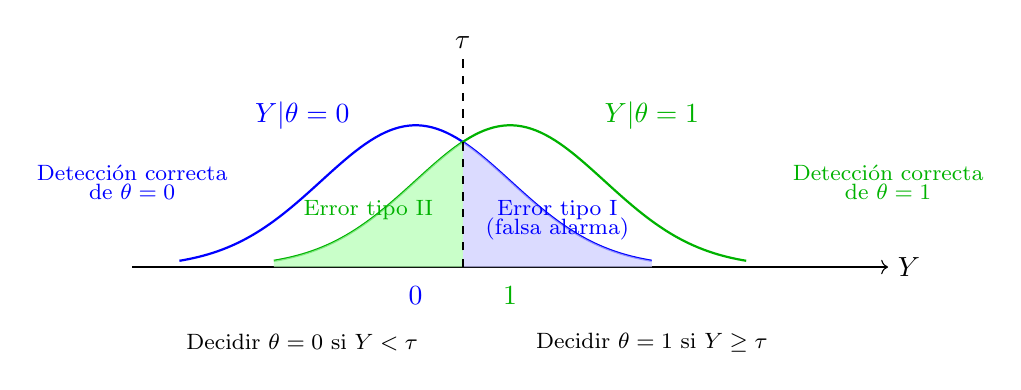
\begin{tikzpicture}[scale=1.2]
    % Eje horizontal
    \draw[->] (-3,0) -- (5,0) node[right] {$Y$};
    
    % Distribución Y|θ=0 (azul) - centrada en 0
    \draw[blue, thick] plot[domain=-2.5:2.5, samples=100] 
      (\x, {1.5*exp(-0.5*\x*\x)});
    \fill[blue!20, opacity=0.7] plot[domain=0.5:2.5, samples=50] 
      (\x, {1.5*exp(-0.5*\x*\x)}) -- (2.5,0) -- (0.5,0) -- cycle;
    
    % Distribución Y|θ=1 (verde) - centrada en 1
    \draw[green!70!black, thick] plot[domain=-1.5:3.5, samples=100] 
      (\x, {1.5*exp(-0.5*(\x-1)*(\x-1))});
    \fill[green!30, opacity=0.7] plot[domain=-1.5:0.5, samples=50] 
      (\x, {1.5*exp(-0.5*(\x-1)*(\x-1))}) -- (0.5,0) -- (-1.5,0) -- cycle;
    
    % Línea de decisión (umbral)
    \draw[dashed, thick] (0.5,0) -- (0.5,2.2) node[above] {$\tau$};
    
    % Etiquetas de las distribuciones
    \node[blue] at (-1.2,1.6) {$Y|\theta=0$};
    \node[green!70!black] at (2.5,1.6) {$Y|\theta=1$};
    
    % Valores de theta en el eje
    \node[blue] at (0,-0.3) {$0$};
    \node[green!70!black] at (1,-0.3) {$1$};
    
    % Etiquetas de probabilidades
    \node[blue] at (-3,1.0) {\footnotesize Detección correcta};
    \node[blue] at (-3,0.8) {\footnotesize de $\theta=0$};
    \node[blue] at (1.5,0.6) {\footnotesize Error tipo I};
    \node[blue] at (1.5,0.4) {\footnotesize (falsa alarma)};
    \node[green!70!black] at (-0.5,0.6) {\footnotesize Error tipo II};
    \node[green!70!black] at (5,1.0) {\footnotesize Detección correcta};
    \node[green!70!black] at (5,0.8) {\footnotesize de $\theta=1$};
    
    % Regiones de decisión
    \node at (-1.2,-0.8) {\footnotesize Decidir $\theta=0$ si $Y < \tau$};
    \node at (2.5,-0.8) {\footnotesize Decidir $\theta=1$ si $Y \geq \tau$};
    
  \end{tikzpicture}
  \caption{Distribuciones condicionales del problema de detección de señal: $Y|\theta=0 \sim \mathcal{N}(0, \sigma_0^2)$ y $Y|\theta=1 \sim \mathcal{N}(1, \sigma_0^2)$ con umbral de decisión $\tau$. Las regiones sombreadas ilustran los errores tipo I (falsa alarma) y tipo II.}
  \label{fig:canal_comunicacion}
  \end{figure}
\end{solution}
%----------------------------
%\question Considere un canal binario simétrico con probabilidad de error $\varepsilon \in (0, 0.5)$, a través del cual se envía una palabra binaria $x = (s_1, \ldots, s_n) \in \{0,1\}^n$, de modo que se recibe la palabra $x = (s_1 \oplus \eta_1, \ldots, s_n \oplus \eta_n)$, donde $\eta_i \sim \text{Bernoulli}(\varepsilon)$ representa el ruido del canal, y $\oplus$ corresponde al operador XOR.
%
%\begin{enumerate}
%    \item Considere la distancia de Hamming, dada por
%    \begin{equation}
%    d(x; y) = \sum_{i=1}^{n} \mathbf{1}(x_i \neq y_i),
%    \end{equation}
%    donde $\mathbf{1}(\cdot)$ es la función indicatriz. Considere que la palabra enviada y recibida son variables aleatorias $S_1^n$ y $X_1^n$, respectivamente, y obtenga una expresión en términos de la distancia de Hamming para la verosimilitud del canal.
%    
%    \item Sea el conjunto $B_k(s) \subset \{0,1\}^n$ dado por
%    \begin{equation}
%    B_k(s) = \{x \in \{0,1\}^n : d(s; x) \leq k\},
%    \end{equation}
%    el cual representa las posibles palabras cuya distancia de Hamming a $s$ es a lo más $k$. Encuentre una expresión para
%    \begin{equation}
%    \eta_k \triangleq P_{X_1^n|S_1^n}(B_k(S_1^n)|S_1^n = (s_1, \ldots, s_n)).
%    \end{equation}
%    
%    \item Considere las siguientes dos hipótesis: si $\theta = 0$ entonces $S_1^n = (0, \ldots, 0)$, y si $\theta = 1$ entonces $S_1^n = (1, \ldots, 1)$. Encuentre un test óptimo $\pi$ para detectar $\theta$ a partir de una medición $x$, cuyo tamaño sea $\alpha_\pi$.
%\end{enumerate}
%----------------------------
%\begin{solution}
%\subsection*{Resolución 3.1}
%
%Notemos que buscamos obtener la verosimilitud, denotada por $f_{X_1^n|S_1^n}(x_1^n|s_1^n)$. Para esto, notemos que, si bien, en general, cada término de la palabra recibida no es necesariamente independiente del resto de símbolos, condicional a la palabra enviada sí lo son, ya que las diferencias símbolo a símbolo estarían explicadas únicamente por los ruidos $\eta_i^n$. Considerando esto, tenemos:
%
%\begin{equation}
%f_{X_1^n|S_1^n}(x_1^n|s_1^n) = \prod_{i=1}^n f_{X_i|S_i}(x_i|s_i).
%\end{equation}
%
%Por otra parte, notemos que el $i$-ésimo símbolo recibido depende, únicamente, del $i$-ésimo símbolo enviado, por lo que condicionar ante la palabra enviada total es equivalente a condicionar, únicamente, ante el $i$-ésimo símbolo, de modo que:
%
%\begin{equation}
%f_{X_1^n|S_1^n}(x_1^n|s_1^n) = \prod_{i=1}^n f_{X_i|S_i}(x_i|s_i).
%\end{equation}

%Luego, dado que $\forall i \in \{1, \ldots, n\}, \eta_i \sim \text{Bernoulli}(\varepsilon)$ tenemos:
%
%\begin{equation}
%f_{X_i|S_i}(x_i|s_i) = \varepsilon \mathbf{1}(x_i \neq s_i) + (1-\varepsilon) \mathbf{1}(x_i = s_i),
%\end{equation}
%
%por lo que:
%
%\begin{equation}
%f_{X_1^n|S_1^n}(x_1^n|s_1^n) = \prod_{i=1}^n [\varepsilon \mathbf{1}(x_i \neq s_i) + (1-\varepsilon) \mathbf{1}(x_i = s_i)].
%\end{equation}
%
%Utilizando intuición, intentemos obtener una expresión sucinta para la multiplicatoria. Notemos que, para cada bit $x_i$, tenemos dos opciones: $x_i = s_i$, en cuyo caso se aporta un término $1-\varepsilon$ a la multiplicatoria; o $x_i \neq s_i$, en cuyo caso se aporta un término $\varepsilon$. Realizando este análisis para todos los bits, $l$ sería el resultado de la multiplicatoria sería de la forma $\varepsilon^l (1-\varepsilon)^{n-l}$, con $D$ el número de bits distintos e $I$ el número de bits iguales entre $x_1^n$ y $s_1^n$. El número de bits distintos está dado por la distancia de Hamming $d(x_1^n; s_1^n)$ entre $x_1^n$ y $s_1^n$, mientras que el número de bits iguales está dado por $n - d(s_1^n; s_1^n)$. Luego, considerando todos los bits, tendríamos las iguales:
%
%\begin{equation}
%f_{X_1^n|S_1^n}(x_1^n|s_1^n) = \prod_{i=1}^n [\varepsilon \mathbf{1}(x_i \neq s_i) + (1-\varepsilon) \mathbf{1}(x_i = s_i)] = \varepsilon^{d(x_1^n;s_1^n)} (1-\varepsilon)^{n-d(x_1^n;s_1^n)}.
%\end{equation}
%
%Sin embargo, notemos que no tenemos una demostración rigurosa de que la expresión obtenida es realmente válida. Para poder validar que realmente se cumple lo planteado, hagamos una demostración por inducción.
%
%Para el caso base $n = 1$, es fácil ver que si los mensajes son iguales tenemos $f_{X_1|S_1}(x_1^1|s_1^1) = 1-\varepsilon$ y, si son distintos, tenemos $f_{X_1|S_1}(x_1^1|s_1^1) = \varepsilon$. Luego, supongamos que la expresión dada se cumple para un $n$ dado.
%
%Para $n+1$ tendremos:
%
%\begin{equation}
%f_{X_1^{n+1}|S_1^{n+1}}(x_1^{n+1}|s_1^{n+1}) = \prod_{i=1}^{n+1} [\varepsilon \mathbf{1}(x_i \neq s_i) + (1-\varepsilon) \mathbf{1}(x_i = s_i)].
%\end{equation}
%
%Si sacamos el término $(n+1)$-ésimo de la multiplicatoria, podemos expresar la probabilidad como:
%
%\begin{equation}
%f_{X_1^{n+1}|S_1^{n+1}}(x_1^{n+1}|s_1^{n+1}) = [\varepsilon \mathbf{1}(x_{n+1} \neq s_{n+1}) + (1-\varepsilon) \mathbf{1}(x_{n+1} = s_{n+1})] f_{X_1^n|S_1^n}(x_1^n|s_1^n).
%\end{equation}
%
%Por la hipótesis inductiva sabemos que se tiene:
%
%\begin{equation}
%f_{X_1^n|S_1^n}(x_1^n|s_1^n) = \prod_{i=1}^n [\varepsilon \mathbf{1}(x_i \neq s_i) + (1-\varepsilon) \mathbf{1}(x_i = s_i)] = \varepsilon^{d(x_1^n;s_1^n)} (1-\varepsilon)^{n-d(x_1^n;s_1^n)},
%\end{equation}

%donde $d(x_1^n; s_1^n)$ correspondería a la distancia de Hamming entre ambas palabras hasta el $n$-ésimo bit, por lo que podemos escribir la ecuación 10 como:
%
%\begin{align}
%f_{X_1^{n+1}|S_1^{n+1}}(x_1^{n+1}|s_1^{n+1}) &= [\varepsilon \mathbf{1}(x_{n+1} \neq s_{n+1}) + (1-\varepsilon) \mathbf{1}(x_{n+1} = s_{n+1})] \varepsilon^{d(x_1^n;s_1^n)} (1-\varepsilon)^{n-d(x_1^n;s_1^n)} \\
%\end{align}
%
%Para proceder, hagamos un análisis por casos en términos de si $x_{n+1}$ y $s_{n+1}$ son iguales o no. Antes de esto, comencemos notando que podemos escribir la distancia de Hamming hasta el término $n+1$ como:
%
%\begin{align}
%d(x_1^{n+1}, s_1^{n+1}) = \sum_{i=1}^{n+1} \mathbf{1}(x_i \neq s_i) &= \mathbf{1}(x_{n+1} \neq s_{n+1}) + \sum_{i=1}^n \mathbf{1}(x_i \neq s_i) \\
%&\Rightarrow d(x_1^{n+1}, s_1^{n+1}) = \mathbf{1}(x_{n+1} \neq s_{n+1}) + d(x_1^n; s_1^n).
%\end{align}
%
%\textbf{Caso 1:} Para el caso 1, supongamos que $x_{n+1} \neq s_{n+1}$. En este caso, por la ecuación 14 podemos ver que $d(x_1^{n+1}, s_1^{n+1}) = d(x_1^n; s_1^n) + 1$. Considerando esto desde de la ecuación 12, tenemos:
%
%\begin{align}
%f_{X_1^{n+1}|S_1^{n+1}}(x_1^{n+1}|s_1^{n+1}) &= [\varepsilon \mathbf{1}(x_{n+1} \neq s_{n+1}) + (1-\varepsilon) \mathbf{1}(x_{n+1} = s_{n+1})] \varepsilon^{d(x_1^n;s_1^n)} (1-\varepsilon)^{n-d(x_1^n;s_1^n)} \\
%&= \varepsilon \varepsilon^{d(x_1^n;s_1^n)} (1-\varepsilon)^{n-d(x_1^n;s_1^n)} \\
%&= \varepsilon^{d(x_1^n;s_1^n)+1} (1-\varepsilon)^{n-d(x_1^n;s_1^n)}
%\end{align}
%
%Notemos que, de acuerdo a lo encontrado, se cumple $d(x_1^n; s_1^n) = d(x_1^{n+1}, s_1^{n+1}) - 1$, por lo que tenemos:
%
%\begin{align}
%f_{X_1^{n+1}|S_1^{n+1}}(x_1^{n+1}|s_1^{n+1}) &= \varepsilon^{d(x_1^{n+1}, s_1^{n+1})} (1-\varepsilon)^{n-d(x_1^{n+1}, s_1^{n+1})+1} \\
%&= \varepsilon^{d(x_1^{n+1}, s_1^{n+1})} (1-\varepsilon)^{n+1-d(x_1^{n+1}, s_1^{n+1})},
%\end{align}
%
%lo cual corresponde a lo que buscábamos demostrar, demostrando que es válido para el caso en que $x_{n+1} \neq s_{n+1}$.
%
%\textbf{Caso 2:} Para el caso 2, supongamos que $x_{n+1} = s_{n+1}$. Con esto, podemos ver que las distancias de Hamming cumplen que $d(x_1^{n+1}, s_1^{n+1}) = d(x_1^n; s_1^n)$. Evaluando en la ecuación 12, tenemos:
%
%\begin{align}
%f_{X_1^{n+1}|S_1^{n+1}}(x_1^{n+1}|s_1^{n+1}) &= [\varepsilon \mathbf{1}(x_{n+1} \neq s_{n+1}) + (1-\varepsilon) \mathbf{1}(x_{n+1} = s_{n+1})] \varepsilon^{d(x_1^n;s_1^n)} (1-\varepsilon)^{n-d(x_1^n;s_1^n)} \\
%&= (1-\varepsilon) \varepsilon^{d(x_1^n;s_1^n)} (1-\varepsilon)^{n-d(x_1^n;s_1^n)} \\
%&= \varepsilon^{d(x_1^n;s_1^n)} (1-\varepsilon)^{n+1-d(x_1^n;s_1^n)} \\
%&= \varepsilon^{d(x_1^{n+1}, s_1^{n+1})} (1-\varepsilon)^{n+1-d(x_1^{n+1}, s_1^{n+1})},
%\end{align}
%
%lo cual, nuevamente, cumple con lo que buscamos demostrar. Esto permite verificar que la expresión encontrada para la probabilidad es válida, por lo que tenemos:
%
%\begin{equation}
%f_{X_1^n|S_1^n}(x_1^n|s_1^n) = \varepsilon^{d(x_1^n;s_1^n)} (1-\varepsilon)^{n-d(x_1^n;s_1^n)}.
%\end{equation}

%\subsection*{Resolución 3.2}
%
%\textbf{Probabilidad de distancia de Hamming}
%
%Durante el desarrollo de la clase me di cuenta que usé la misma variable tanto para el ruido como para la probabilidad. Por lo tanto, la variable de la probabilidad la reemplacé por $\eta_k$, de modo que:
%
%\begin{equation}
%\eta_k(s_1^n) \triangleq P_{X_1^n|S_1^n}(X_1^n \in B_k(S_1^n)|S_1^n = s_1^n).
%\end{equation}
%
%Para obtener la expresión solicitada, comencemos notando que podemos separar el conjunto $B_k(s_1^n)$ como:
%
%\begin{equation}
%B_k(s_1^n) = \{x_1^n \in \{0,1\}^n | d(x_1^n; s_1^n) \leq k\} = \bigcup_{i=0}^k \{x_1^n \in \{0,1\}^n | d(x_1^n; s_1^n) = i\},
%\end{equation}
%
%donde $\forall i, j, C_i(s_1^n) \cap C_j(s_1^n) = \emptyset$ por lo que $C_i(s_1^n)$ y $C_j(s_1^n)$ son disjuntos. La forma en que podemos interpretar cada $C_i(s_1^n)$ es el conjunto de posibles palabras $x^n$ que están a una distancia de Hamming $i$ de la palabra $s_1^n$, y, por ende, $B_k(s_1^n)$ correspondería al conjunto de palabras con distancia de Hamming menor o igual a $k$.
%
%Luego, dado que los conjuntos son disjuntos, podemos escribir $\eta_k(s_1^n)$ como:
%
%\begin{equation}
%\eta_k(s_1^n) = P_{X_1^n|S_1^n}(X_1^n \in B_k(S_1^n)|S_1^n = s_1^n) = \sum_{i=0}^k P_{X_1^n|S_1^n}(X_1^n \in C_i(S_1^n)|S_1^n = s_1^n).
%\end{equation}
%
%Por la forma en que está definido cada conjunto $C_i$, podemos escribir cada una de las probabilidades $P_{X_1^n|S_1^n}(X_1^n \in C_i(S_1^n)|S_1^n = s_1^n)$ como:
%
%\begin{equation}
%P_{X_1^n|S_1^n}(X_1^n \in C_i(S_1^n)|S_1^n = s_1^n) = P_{X_1^n|S_1^n}(d(X_1^n; S_1^n) = i|S_1^n = s_1^n)
%\end{equation}
%
%donde, reemplazando la definición de la distancia de Hamming, tenemos:
%
%\begin{equation}
%P_{X_1^n|S_1^n}(X_1^n \in C_i(S_1^n)|S_1^n = s_1^n) = P_{X_1^n|S_1^n}\left(\sum_{j=1}^n \mathbf{1}(X_j \neq S_j) = i|S_1^n = s_1^n\right).
%\end{equation}
%
%Luego, notemos que, para cada término de la sumatoria, al condicionar ante $S_1^n = s_1^n$ podemos ver que se tiene $\mathbf{1}(X_j \neq S_j) = \mathbf{1}(s_j \neq \eta_j \neq s_j) = \mathbf{1}(\eta_j = 1)$, donde, dado que $\eta_j \in \{0,1\}$, tenemos $\mathbf{1}(\eta_j = 1) = \eta_j$, de modo que podemos escribir la probabilidad anterior en términos de cada término del ruido como:
%
%\begin{equation}
%P_{X_1^n|S_1^n}(X_1^n \in C_i(S_1^n)|S_1^n = s_1^n) = P_{\eta}\left(\sum_{j=1}^n \eta_j = i\right).
%\end{equation}

%Luego, dado que $\forall j \in \{1, \ldots, n\}, \eta_j \sim \text{Bernoulli}(\varepsilon)$, y dado que los ruidos son i.i.d., por propiedades de la distribución Bernoulli sabemos que $\sum_{j=1}^n \eta_j \sim \text{Binomial}(n, \varepsilon)$, por lo que:
%
%\begin{equation}
%P_{\eta}\left(\sum_{j=1}^n \eta_j = i\right) = \binom{n}{i} \varepsilon^i (1-\varepsilon)^{n-i}.
%\end{equation}
%
%Así, tenemos:
%
%\begin{equation}
%P_{X_1^n|S_1^n}(X_1^n \in C_i(S_1^n)|S_1^n = s_1^n) = \binom{n}{i} \varepsilon^i (1-\varepsilon)^{n-i},
%\end{equation}
%
%de modo que:
%
%\begin{equation}
%\eta_k(s_1^n) = \sum_{i=0}^k \binom{n}{i} \varepsilon^i (1-\varepsilon)^{n-i}.
%\end{equation}

%\subsection*{Resolución 3.3}
%
%Para plantear la regla óptima, notemos que, por lema de Neyman-Pearson, sabemos que cualquier regla óptima sería de la forma:
%
%\begin{equation}
%\pi^*(\rho, X_1^n) = \begin{cases}
%1 & \text{si } L(X_1^n|\theta = 1) > \nu L(X_1^n|\theta = 0) \\
%\rho & \text{si } L(X_1^n|\theta = 1) = \nu L(X_1^n|\theta = 0) \\
%0 & \text{si } L(X_1^n|\theta = 1) < \nu L(X_1^n|\theta = 0)
%\end{cases}
%\end{equation}
%
%donde $L(X_1^n|\theta)$ corresponde a la verosimilitud que encontramos anteriormente, donde, tomando en consideración que si $\theta = 0$ entonces $S_1^n = (0, \ldots, 0) \triangleq s_0$ y si $\theta = 1$ entonces $S_1^n = (1, \ldots, 1) \triangleq s_1$, podemos ver que:
%
%\begin{align}
%L(X_1^n|\theta = 1) &= \varepsilon^{d(X_1^n;s_1)} (1-\varepsilon)^{n-d(X_1^n;s_1)} \\
%L(X_1^n|\theta = 0) &= \varepsilon^{d(X_1^n;s_0)} (1-\varepsilon)^{n-d(X_1^n;s_0)}.
%\end{align}
%
%Si, además, denotamos $\ell(X_1^n)$ a la razón de verosimilitud, dada por:
%
%\begin{equation}
%\ell(X_1^n) \triangleq \frac{L(X_1^n|\theta = 1)}{L(X_1^n|\theta = 0)},
%\end{equation}

%podemos replantear la regla óptima como:
%
%\begin{equation}
%\pi^*(\rho, X_1^n) = \begin{cases}
%1 & \text{si } \ell(X_1^n) > \nu \\
%\rho & \text{si } \ell(X_1^n) = \nu \\
%0 & \text{si } \ell(X_1^n) < \nu
%\end{cases}
%\end{equation}
%
%Para desarrollar la razón de verosimilitud, comencemos analizando las distancias de Hamming a cada palabra de la codificación. Notemos que:
%
%\begin{align}
%d(X_1^n; s_0) &= \sum_{i=1}^n \mathbf{1}(X_i \neq 0) \\
%d(X_1^n; s_1) &= \sum_{i=1}^n \mathbf{1}(X_i \neq 1),
%\end{align}
%
%por lo que:
%
%\begin{equation}
%d(X_1^n; s_0) + d(X_1^n; s_1) = \sum_{i=1}^n [\mathbf{1}(X_i \neq 0) + \mathbf{1}(X_i \neq 1)] = n,
%\end{equation}
%
%de modo que se tiene $d(X_1^n; s_0) = n - d(X_1^n; s_1)$ y $d(X_1^n; s_0) = n - d(X_1^n; s_1)$.
%
%Luego, desarrollemos la razón de verosimilitud, tratando de dejar todo en función de la distancia a la palabra $s_0$. Al hacerlo, tenemos:
%
%\begin{align}
%\ell(X_1^n) &= \frac{\varepsilon^{d(X_1^n;s_1)} (1-\varepsilon)^{n-d(X_1^n;s_1)}}{\varepsilon^{d(X_1^n;s_0)} (1-\varepsilon)^{n-d(X_1^n;s_0)}} \\
%&= \frac{\varepsilon^{n-d(X_1^n;s_0)} (1-\varepsilon)^{d(X_1^n;s_0)}}{\varepsilon^{d(X_1^n;s_0)} (1-\varepsilon)^{n-d(X_1^n;s_0)}} \\
%&= \left(\frac{1-\varepsilon}{\varepsilon}\right)^{2d(X_1^n;s_0)-n}.
%\end{align}
%
%Así, si nos enfocamos en el caso donde $\pi^*(\rho, X_1^n) = 1$, teniendo en consideración que los otros dos casos serían análogos, notemos que $\pi^*(\rho, X_1^n) = 1$ ssi $\ell(X_1^n) > \nu$:
%
%\begin{align}
%&\Leftrightarrow \left(\frac{1-\varepsilon}{\varepsilon}\right)^{2d(X_1^n;s_0)-n} > \nu \\
%&\Leftrightarrow (2d(X_1^n; s_0) - n) \log\left(\frac{1-\varepsilon}{\varepsilon}\right) > \log(\nu).
%\end{align}
%
%Si despejamos la distancia a la palabra $s_0$, tenemos:
%
%\begin{equation}
%d(X_1^n; s_0) > \frac{n}{2} + \frac{\log(\nu)}{2\log\left(\frac{1-\varepsilon}{\varepsilon}\right)},
%\end{equation}
%
%de modo que la regla óptima es de la forma:
%
%\begin{equation}
%\pi^*(\rho, X_1^n) = \begin{cases}
%1 & \text{si } d(X_1^n; s_0) > \frac{n}{2} + \frac{\log(\nu)}{2\log\left(\frac{1-\varepsilon}{\varepsilon}\right)} \\
%\rho & \text{si } d(X_1^n; s_0) = \frac{n}{2} + \frac{\log(\nu)}{2\log\left(\frac{1-\varepsilon}{\varepsilon}\right)} \\
%0 & \text{si } d(X_1^n; s_0) < \frac{n}{2} + \frac{\log(\nu)}{2\log\left(\frac{1-\varepsilon}{\varepsilon}\right)}
%\end{cases}
%\end{equation}

%Por último, queremos que el tamaño del test sea igual a un cierto valor $\alpha$ arbitrario, para lo cual, si consideramos que $\rho \sim \text{Bernoulli}(p)$, debemos determinar los valores de $p$ y $\nu$ tales que $\alpha_{\pi^*} = \alpha$. Comencemos notando que el tamaño del test corresponde a:
%
%\begin{equation}
%\alpha_{\pi^*} = E_{\theta,X_1^n}[\pi^*(\rho, X_1^n)|\theta = 0],
%\end{equation}
%
%lo cual se puede reescribir como:
%
%\begin{equation}
%\alpha_{\pi^*} = P_{X_1^n}(\ell(X_1^n) > \nu|\theta = 0) + p P_{X_1^n}(\ell(X_1^n) = \nu|\theta = 0).
%\end{equation}
%
%Expresemos cada término por separado. Comenzando por el término de la izquierda, tenemos:
%
%\begin{equation}
%P_{X_1^n}(\ell(X_1^n) > \nu|\theta = 0) = P_{X_1^n}(d(X_1^n; s_0) > \tau(\nu)|\theta = 0) = 1 - P_{X_1^n}(d(X_1^n; s_0) \leq \tau(\nu)|\theta = 0),
%\end{equation}
%
%donde:
%
%\begin{equation}
%\tau(\nu) \triangleq \frac{n}{2} + \frac{\log(\nu)}{2\log\left(\frac{1-\varepsilon}{\varepsilon}\right)}
%\end{equation}
%
%denota el umbral utilizado. Podemos ver que la probabilidad corresponde a $\gamma_{\tau(\nu)}(s_0)$ calculado anteriormente, donde tomamos el piso de $\tau(\nu)$ dado que, en general, este puede ser cualquier número real. De este modo, tenemos:
%
%\begin{equation}
%P_{X_1^n}(\ell(X_1^n) > \nu|\theta = 0) = 1 - \gamma_{\lfloor\tau(\nu)\rfloor}(s_0).
%\end{equation}
%
%Por otra parte, para el término de la derecha tenemos:
%
%\begin{equation}
%P_{X_1^n}(\ell(X_1^n) = \nu|\theta = 0) = P_{X_1^n}(d(X_1^n; s_0) = \tau(\nu)|\theta = 0).
%\end{equation}
%
%Notemos que, dependiendo de si $\tau(\nu)$ es un número natural o no, esta probabilidad puede o no tomar un valor. En particular, si $\tau(\nu)$ no es un número natural, entonces la probabilidad es 0, mientras que si es un número natural, la probabilidad correspondería a:
%
%\begin{equation}
%P_{X_1^n}(\ell(X_1^n) = \nu|\theta = 0) = \left(\frac{n}{\tau(\nu)}\right) \varepsilon^{\tau(\nu)} (1-\varepsilon)^{n-\tau(\nu)} \mathbf{1}_{\mathbb{N}}(\tau(\nu)).
%\end{equation}
%
%Podemos juntar estos dos casos utilizando una indicatriz, de modo que:
%
%\begin{equation}
%P_{X_1^n}(\ell(X_1^n) = \nu|\theta = 0) = \left(\frac{n}{\tau(\nu)}\right) \varepsilon^{\tau(\nu)} (1-\varepsilon)^{n-\tau(\nu)} \mathbf{1}_{\mathbb{N}}(\tau(\nu)).
%\end{equation}
%
%Así, tenemos que el tamaño de la regla óptima está dado por:
%
%\begin{equation}
%\alpha_{\pi^*} = 1 - \gamma_{\lfloor\tau(\nu)\rfloor}(s_0) + p \left(\frac{n}{\tau(\nu)}\right) \varepsilon^{\tau(\nu)} (1-\varepsilon)^{n-\tau(\nu)} \mathbf{1}_{\mathbb{N}}(\tau(\nu)),
%\end{equation}
%
%por lo que el objetivo sería encontrar $p$ y $\nu$ tales que:
%
%\begin{equation}
%1 - \gamma_{\lfloor\tau(\nu)\rfloor}(s_0) + p \left(\frac{n}{\tau(\nu)}\right) \varepsilon^{\tau(\nu)} (1-\varepsilon)^{n-\tau(\nu)} \mathbf{1}_{\mathbb{N}}(\tau(\nu)) = \alpha_{\pi^*}.
%\end{equation}
%
%Sin embargo, podemos ver que las relaciones que se tienen no son invertibles, por lo que no sería posible encontrar los parámetros de forma analítica y, para poder hacerlo, sería necesario recurrir a técnicas numéricas, ya sea resolviendo la ecuación 58 numéricamente o construyendo una curva ROC y, a partir de esta, determinando el valor de los parámetros.
%\end{solution}
%----------------------------
\question Una máquina de acuñación defectuosa produce monedas cuya probabilidad de obtener cara es una variable aleatoria $P$ con PDF
\begin{equation}
f_P(p) = \begin{cases}
1 + \sin(2\pi p), & \text{si } p \in [0,1], \\
0, & \text{en otro caso}.
\end{cases}
\end{equation}

En esencia, una moneda específica producida por esta máquina tendrá una probabilidad fija $P = p$ de dar cara, pero usted no conoce inicialmente cuál es esa probabilidad. Una moneda producida por esta máquina es seleccionada y lanzada repetidamente, con lanzamientos sucesivos asumidos independientes.

\begin{enumerate}
    \item Encuentre la probabilidad de que el primer lanzamiento de la moneda resulte en cara.
    
    \item Dado que el primer lanzamiento de la moneda resultó en cara, encuentre la PDF condicional de $P$.
    
    \item Dado que el primer lanzamiento de la moneda resultó en cara, encuentre la probabilidad condicional de obtener cara en el segundo lanzamiento.
\end{enumerate}
%----------------------------
\begin{solution}
  \subsection*{Resolución 3.1}

Primero, es crucial entender qué representa cada elemento del problema:

\begin{itemize}
\item \textbf{La variable $P$:} No es un número fijo, sino una \emph{variable aleatoria} que representa la probabilidad de obtener cara de una moneda específica producida por la máquina defectuosa. Cada moneda que produce la máquina tiene su propia probabilidad $P$ de dar cara, pero esta probabilidad varía de moneda a moneda.

\item \textbf{La distribución $f_P(p) = 1 + \sin(2\pi p)$:} Esta función nos dice qué tan probable es que una moneda producida por la máquina tenga probabilidad $p$ de dar cara. Es una distribución que:
\begin{itemize}
\item Oscila entre $1 - 1 = 0$ y $1 + 1 = 2$
\item Tiene máximos en $p = 0.25$ y $p = 0.75$ (donde $\sin(2\pi p) = 1$)
\item Tiene mínimos en $p = 0$ y $p = 0.5$ y $p = 1$ (donde $\sin(2\pi p) = 0$ o $-1$)
\item Esto significa que la máquina tiende a producir monedas sesgadas hacia $p = 0.25$ o $p = 0.75$, pero raramente produce monedas justas ($p = 0.5$)
\end{itemize}

\item \textbf{El proceso:} Tomamos una moneda al azar de las producidas por esta máquina defectuosa. No sabemos cuál es su probabilidad específica $P$, solo sabemos que sigue la distribución dada.
\end{itemize}

El problema fundamental aquí es que no conocemos el valor exacto de la probabilidad $P$ de la moneda específica que tenemos. Esto significa que debemos considerar todos los posibles valores que $P$ puede tomar, ponderando cada uno por su probabilidad de ocurrencia según la distribución $f_P(p)$ que nos proporciona el enunciado.

Para calcular la probabilidad $\mathbb{P}(A)$, usamos la versión continua del teorema de probabilidad total:

\begin{equation}
\mathbb{P}(A) = \int_0^1 \mathbb{P}(A | P = p)f_P(p) \, dp = \int_0^1 p(1 + \sin(2\pi p)) \, dp,
\end{equation}

donde $\mathbb{P}(A | P = p) = p$ porque si la moneda tiene probabilidad fija $p$ de dar cara, entonces la probabilidad de obtener cara es exactamente $p$. Separamos la integral en dos partes:
\begin{equation}
\mathbb{P}(A) = \int_0^1 p \, dp + \int_0^1 p \sin(2\pi p) \, dp
\end{equation}

La primera integral es directa:
\begin{equation}
\int_0^1 p \, dp = \left[\frac{p^2}{2}\right]_0^1 = \frac{1^2}{2} - \frac{0^2}{2} = \frac{1}{2}
\end{equation}


Para la segunda integral, $\int_0^1 p \sin(2\pi p) \, dp$, usamos integración por partes con:
\begin{align}
u &= p \quad \Rightarrow \quad du = dp \\
dv &= \sin(2\pi p) \, dp \quad \Rightarrow \quad v = -\frac{1}{2\pi}\cos(2\pi p)
\end{align}

Aplicando la fórmula de integración por partes $\int u \, dv = uv - \int v \, du$:
\begin{align}
\int_0^1 p \sin(2\pi p) \, dp &= \left[p \cdot \left(-\frac{1}{2\pi}\cos(2\pi p)\right)\right]_0^1 - \int_0^1 \left(-\frac{1}{2\pi}\cos(2\pi p)\right) dp \\
&= \left[-\frac{p}{2\pi}\cos(2\pi p)\right]_0^1 + \frac{1}{2\pi}\int_0^1 \cos(2\pi p) \, dp
\end{align}

Evaluamos cada término por separado:
\begin{itemize}
  \item \textbf{Primer término:}
\begin{align}
\left[-\frac{p}{2\pi}\cos(2\pi p)\right]_0^1 &= -\frac{1}{2\pi}\cos(2\pi \cdot 1) - \left(-\frac{0}{2\pi}\cos(2\pi \cdot 0)\right) \\
&= -\frac{1}{2\pi}\cos(2\pi) - 0 \\
&= -\frac{1}{2\pi} \cdot 1 = -\frac{1}{2\pi}
\end{align}

donde usamos que $\cos(2\pi) = 1$.

\item \textbf{Segundo término:}
\begin{align}
\frac{1}{2\pi}\int_0^1 \cos(2\pi p) \, dp &= \frac{1}{2\pi} \left[\frac{1}{2\pi}\sin(2\pi p)\right]_0^1 \\
&= \frac{1}{(2\pi)^2}[\sin(2\pi \cdot 1) - \sin(2\pi \cdot 0)] \\
&= \frac{1}{4\pi^2}[0 - 0] = 0
\end{align}

donde usamos que $\sin(2\pi) = \sin(0) = 0$.
\end{itemize}
Por tanto:
\begin{equation}
\int_0^1 p \sin(2\pi p) \, dp = -\frac{1}{2\pi} + 0 = -\frac{1}{2\pi}
\end{equation}

Combinando ambas integrales:
\begin{align}
\mathbb{P}(A) &= \int_0^1 p \, dp + \int_0^1 p \sin(2\pi p) \, dp \\
&= \frac{1}{2} + \left(-\frac{1}{2\pi}\right) \\
&= \frac{1}{2} - \frac{1}{2\pi} \\
&= \frac{\pi - 1}{2\pi} \approx 0.341
\end{align}


El resultado $\mathbb{P}(A) = \frac{\pi - 1}{2\pi} \approx 0.341 < 0.5$ tiene sentido intuitivo:

\begin{itemize}
\item Si todas las monedas fueran justas ($P = 0.5$ siempre), tendríamos $\mathbb{P}(A) = 0.5$
\item Si la distribución fuera uniforme ($f_P(p) = 1$), también tendríamos $\mathbb{P}(A) = 0.5$
\item Pero nuestra distribución $f_P(p) = 1 + \sin(2\pi p)$ favorece valores como $p = 0.25$ y $p = 0.75$
\item El término $-\frac{1}{2\pi}$ proviene del componente sinusoidal y refleja el sesgo de la distribución
\item Como la distribución le da más peso relativo a monedas con probabilidades menores (especialmente $p = 0.25$), el resultado global es menor que $0.5$
\end{itemize}\subsection*{Resolución 3.2}

Imagina que inicialmente no sabemos nada específico sobre nuestra moneda, solo que viene de la máquina defectuosa. Pero cuando lanzamos la moneda y sale cara, esta observación nos da información valiosa

\begin{itemize}
\item \textbf{Antes del lanzamiento:} Cualquier moneda podría tener probabilidades desde $p = 0$ hasta $p = 1$, pero algunas son más probables según $f_P(p) = 1 + \sin(2\pi p)$
\item \textbf{Después de observar cara:} Las monedas con $p$ muy pequeño (digamos $p = 0.1$) se vuelven menos creíbles, mientras que las monedas con $p$ más grande (digamos $p = 0.8$) se vuelven más creíbles
\item Esto porque si una moneda tiene $p = 0.1$, es muy raro que dé cara, pero si tiene $p = 0.8$, es bastante común que dé cara
\end{itemize}

La situación cambia fundamentalmente cuando observamos que el primer lanzamiento dio cara. Esta nueva información nos permite actualizar nuestro conocimiento sobre la distribución de $P$ usando inferencia bayesiana. La observación nos proporciona evidencia que modifica nuestra creencia inicial sobre qué valores de $P$ son más probables.

Recordemos que la regla de Bayes viene dada por:
\begin{equation}
\mathbb{P}(H | E) = \frac{\mathbb{P}(E | H) \mathbb{P}(H)}{\mathbb{P}(E)}
\end{equation}
donde $H$ es una hipótesis (en este caso, un valor específico de $P$) y $E$ es la evidencia observada (el evento de obtener cara). Usando la regla de Bayes para encontrar la distribución posterior de $P$ dado que observamos cara:

\begin{equation}
f_{P|A}(p) = \frac{\mathbb{P}(A | P = p)f_P(p)}{\mathbb{P}(A)}
\end{equation}

Donde:
\begin{itemize}
\item $\mathbb{P}(A | P = p) = p$ (si la moneda tiene probabilidad $p$, entonces la probabilidad de cara es $p$)
\item $f_P(p) = 1 + \sin(2\pi p)$ (distribución original de la máquina)
\item $\mathbb{P}(A) = \frac{\pi - 1}{2\pi}$ (calculado en la parte anterior)
\end{itemize}

Sustituyendo:
\begin{equation}
f_{P|A}(p) = \frac{p \cdot (1 + \sin(2\pi p))}{\frac{\pi - 1}{2\pi}} = \frac{2\pi p(1 + \sin(2\pi p))}{\pi - 1}
\end{equation}

Por tanto:
\begin{equation}
f_{P|A}(p) = \begin{cases}
\frac{2\pi p(1 + \sin(2\pi p))}{\pi - 1}, & \text{si } 0 \leq p \leq 1, \\
0, & \text{en otro caso}.
\end{cases}
\end{equation}

Comparando $f_{P|A}(p)$ con la distribución original $f_P(p)$:
\begin{itemize}
\item La nueva distribución tiene un factor adicional de $p$ en el numerador
\item Esto significa que valores más grandes de $p$ reciben mayor peso relativo
\item Por ejemplo: si $p = 0.1$, el factor $p = 0.1$ reduce la probabilidad; si $p = 0.8$, el factor $p = 0.8$ la aumenta considerablemente
\item Después de observar una cara, es más probable que nuestra moneda tenga una probabilidad alta de dar cara
\end{itemize}

\subsection*{Resolución 3.3}

Ahora queremos predecir el segundo lanzamiento, pero con una ventaja: \emph{ya sabemos que el primer lanzamiento dio cara}. Esta información cambia todo nuestro análisis.


\begin{itemize}
\item \textbf{Situación inicial:} Tenemos una moneda de la máquina defectuosa y el primer lanzamiento dio cara
\item \textbf{Lo que sabemos ahora:} Gracias al primer lanzamiento, tenemos una mejor idea de qué tipo de moneda es (distribución actualizada $f_{P|A}(p)$)
\item \textbf{Lo que queremos:} La probabilidad de que el segundo lanzamiento también sea cara
\item \textbf{Clave importante:} Los lanzamientos son independientes \emph{dado el valor de $P$}, pero como no conocemos $P$ exactamente, hay dependencia estadística entre los lanzamientos
\end{itemize}

Para predecir el resultado del segundo lanzamiento, debemos utilizar toda la información disponible. Esto significa que ya no usamos la distribución original $f_P(p)$, sino la distribución actualizada $f_{P|A}(p)$ que incorpora la información del primer lanzamiento. 

Es importante recordar que los lanzamientos son independientes condicionalmente a $P$, lo que significa que una vez que conocemos (o tenemos una distribución sobre) el valor de $P$, los resultados de diferentes lanzamientos no se influyen mutuamente. Tenemos:
\begin{align}
\mathbb{P}(B | A) &= \int_0^1 \mathbb{P}(B | P = p, A)f_{P|A}(p) \, dp \\
&= \int_0^1 \mathbb{P}(B | P = p)f_{P|A}(p) \, dp \\
&= \frac{2\pi}{\pi - 1} \int_0^1 p^2(1 + \sin(2\pi p)) \, dp.
\end{align}

\textbf{Explicación de cada paso:}
\begin{itemize}
\item \textbf{Primera línea:} Usamos el teorema de probabilidad total, pero ahora con la distribución actualizada $f_{P|A}(p)$
\item \textbf{Segunda línea:} Aplicamos independencia condicional: $\mathbb{P}(B | P = p, A) = \mathbb{P}(B | P = p) = p$
\item \textbf{¿Por qué independencia condicional?} Si sabemos que $P = p$, entonces el resultado del primer lanzamiento no afecta directamente al segundo; ambos solo dependen de $p$
\item \textbf{Tercera línea:} Sustituimos $f_{P|A}(p) = \frac{2\pi p(1 + \sin(2\pi p))}{\pi - 1}$
\end{itemize}


Observa que ahora tenemos $p^2$ en la integral (comparado con solo $p$ en la parte (a)). Este $p^2$ proviene de:
\begin{itemize}
\item Un factor $p$ de $\mathbb{P}(B | P = p) = p$ (probabilidad del segundo lanzamiento)
\item Un factor $p$ de $f_{P|A}(p)$ (la actualización bayesiana que favorece valores grandes de $p$)
\end{itemize}

Necesitamos calcular:
\begin{equation}
\int_0^1 p^2(1 + \sin(2\pi p)) \, dp
\end{equation}

Separamos la integral en dos partes:
\begin{equation}
\int_0^1 p^2(1 + \sin(2\pi p)) \, dp = \int_0^1 p^2 \, dp + \int_0^1 p^2 \sin(2\pi p) \, dp
\end{equation}

\textbf{Primera integral:}
\begin{equation}
\int_0^1 p^2 \, dp = \left[\frac{p^3}{3}\right]_0^1 = \frac{1^3}{3} - \frac{0^3}{3} = \frac{1}{3}
\end{equation}

\textbf{Segunda integral:}
Para $\int_0^1 p^2 \sin(2\pi p) \, dp$, usamos integración por partes dos veces.

\begin{align}
u &= p^2 \quad \Rightarrow \quad du = 2p \, dp \\
dv &= \sin(2\pi p) \, dp \quad \Rightarrow \quad v = -\frac{1}{2\pi}\cos(2\pi p)
\end{align}

\begin{align}
\int_0^1 p^2 \sin(2\pi p) \, dp &= \left[p^2 \cdot \left(-\frac{1}{2\pi}\cos(2\pi p)\right)\right]_0^1 - \int_0^1 \left(-\frac{1}{2\pi}\cos(2\pi p)\right) \cdot 2p \, dp \\
&= \left[-\frac{p^2}{2\pi}\cos(2\pi p)\right]_0^1 + \frac{1}{\pi}\int_0^1 p \cos(2\pi p) \, dp
\end{align}

Evaluando el primer término:
\begin{align}
\left[-\frac{p^2}{2\pi}\cos(2\pi p)\right]_0^1 &= -\frac{1^2}{2\pi}\cos(2\pi) - \left(-\frac{0^2}{2\pi}\cos(0)\right) \\
&= -\frac{1}{2\pi} \cdot 1 - 0 = -\frac{1}{2\pi}
\end{align}

\textbf{Segunda integración por partes} para $\int_0^1 p \cos(2\pi p) \, dp$:
\begin{align}
u &= p \quad \Rightarrow \quad du = dp \\
dv &= \cos(2\pi p) \, dp \quad \Rightarrow \quad v = \frac{1}{2\pi}\sin(2\pi p)
\end{align}

\begin{align}
\int_0^1 p \cos(2\pi p) \, dp &= \left[p \cdot \frac{1}{2\pi}\sin(2\pi p)\right]_0^1 - \int_0^1 \frac{1}{2\pi}\sin(2\pi p) \, dp \\
&= \left[\frac{p}{2\pi}\sin(2\pi p)\right]_0^1 + \frac{1}{2\pi}\int_0^1 \sin(2\pi p) \, dp \\
&= 0 + \frac{1}{2\pi} \left[-\frac{1}{2\pi}\cos(2\pi p)\right]_0^1 \\
&= -\frac{1}{4\pi^2}[\cos(2\pi) - \cos(0)] = -\frac{1}{4\pi^2}[1 - 1] = 0
\end{align}

Por tanto:
\begin{equation}
\int_0^1 p^2 \sin(2\pi p) \, dp = -\frac{1}{2\pi} + \frac{1}{\pi} \cdot 0 = -\frac{1}{2\pi}
\end{equation}

Combinando ambas integrales:
\begin{align}
\int_0^1 p^2(1 + \sin(2\pi p)) \, dp &= \int_0^1 p^2 \, dp + \int_0^1 p^2 \sin(2\pi p) \, dp \\
&= \frac{1}{3} + \left(-\frac{1}{2\pi}\right) \\
&= \frac{1}{3} - \frac{1}{2\pi} \\
&= \frac{2\pi - 3}{6\pi}
\end{align}

Finalmente, sustituimos este resultado en la expresión para $\mathbb{P}(B | A)$:
\begin{align}
\mathbb{P}(B | A) &= \frac{2\pi}{\pi - 1} \cdot \frac{2\pi - 3}{6\pi} \\
&= \frac{2\pi(2\pi - 3)}{6\pi(\pi - 1)} \\
&= \frac{2(2\pi - 3)}{6(\pi - 1)} \\
&= \frac{2\pi - 3}{3(\pi - 1)} \\
&= \frac{2\pi - 3}{3\pi - 3} \approx 0.5110
\end{align}


El resultado $0.5110 > 0.5$ confirma nuestra intuición y tiene mucho sentido:
\begin{itemize}
\item \textbf{Comparación:} Recuerda que $\mathbb{P}(A) = \frac{\pi-1}{2\pi} \approx 0.341 < 0.5$
\item \textbf{Efecto del aprendizaje:} Después de observar cara, nuestra estimación sube de $0.341$ a $0.511$
\item \textbf{¿Por qué es mayor que 0.5?} El primer lanzamiento nos dio evidencia de que probablemente tenemos una moneda con $p > 0.5$
\item \textbf{Dependencia estadística:} Aunque los lanzamientos son físicamente independientes, estadísticamente están correlacionados a través de nuestro desconocimiento de $P$
\end{itemize}
\end{solution}
%----------------------------
\question El negocio ``Donde la Sonia'' tiene $N$ clientes regulares, donde $N$ es una variable aleatoria con PMF
\begin{equation}
p_N(n) = p^{n-1}(1-p) \quad \text{para } n = 1, 2, 3, \ldots
\end{equation}

Cada viernes por la noche, el negocio organiza una promoción especial. Cada cliente regular decide asistir a la promoción con probabilidad $q$, independientemente de todos los otros clientes. Si un cliente asiste a la promoción, entonces gasta una cantidad de dinero $M$, que es una variable aleatoria continua con PDF
\begin{equation}
f_M(m) = \lambda e^{-\lambda m} \quad \text{para } m \geq 0.
\end{equation}

$N$, $M$, y si cada cliente asiste son todos independientes. Determine:

\begin{enumerate}
    \item La esperanza y varianza del número de clientes que asisten a la promoción.
    
    \item \textbf{[Propuesto]}La esperanza y varianza de la cantidad total de dinero gastada en la promoción.
\end{enumerate}
%----------------------------
\begin{solution}
\subsection*{Resolución 4.1}

Este problema presenta una situación  de aleatoriedad compuesta que es muy común en la vida real. Imagina la situación del negocio ``Donde la Sonia'': tenemos dos fuentes de incertidumbre que se combinan. Primero, no sabemos cuántos clientes regulares tiene el negocio, este número $N$ es aleatorio y sigue una distribución geométrica. Segundo, cada cliente decide independientemente si asistir o no a la promoción con probabilidad $q$. El resultado final es que el número de asistentes $K$ depende de ambas fuentes de incertidumbre, creando una estructura de dependencia compleja.

La distribución geométrica $p_N(n) = p^{n-1}(1-p)$ modela situaciones donde contamos ``hasta el primer éxito''. En nuestro contexto, podemos interpretarla como el número de clientes que el negocio puede mantener antes de que algún factor externo (competencia, cambio de ubicación, etc.) cause una ``pérdida''.

Primero identifiquemos todas nuestras variables aleatorias y sus propiedades:

\begin{itemize}
\item $N$: Número de clientes regulares (distribución geométrica)
\item $B$: Variable Bernoulli que indica si un cliente asiste ($B = 1$) o no ($B = 0$)
\item $M$: Cantidad gastada por un cliente que asiste (distribución exponencial)
\item $K$: Número total de clientes que asisten a la promoción
\end{itemize}

Las propiedades de estas distribuciones son:

\begin{align}
\mathbb{E}[N] &= \frac{1}{1-p}, & \text{var}(N) &= \frac{p}{(1-p)^2}, \\
\mathbb{E}[M] &= \frac{1}{\lambda}, & \text{var}(M) &= \frac{1}{\lambda^2}, \\
\mathbb{E}[B] &= q, & \text{var}(B) &= q(1-q).
\end{align}


Para entender mejor estos valores, consideremos algunos ejemplos: si $p = 0.1$, entonces $\mathbb{E}[N] = \frac{1}{0.9} \approx 1.11$ clientes en promedio; si $p = 0.5$, entonces $\mathbb{E}[N] = 2$ clientes en promedio; y si $p = 0.9$, entonces $\mathbb{E}[N] = 10$ clientes en promedio. Notemos que la varianza crece considerablemente cuando $p$ se acerca a 1.



El número de clientes que asisten es una suma aleatoria: $K = B_1 + B_2 + \cdots + B_N$. Esto significa que cada $B_i$ es una variable Bernoulli independiente (el cliente $i$ asiste con probabilidad $q$), pero el número de términos $N$ también es aleatorio. Esta es la esencia de una ``suma aleatoria'': sumamos un número aleatorio de variables aleatorias.

Una suma aleatoria tiene la forma general $S = X_1 + X_2 + \cdots + X_N$, donde $N$ es una variable aleatoria independiente de las $X_i$, y todas las $X_i$ son independientes e idénticamente distribuidas. Para entender de dónde salen las fórmulas, consideremos que condicionalmente a $N = n$, tenemos una suma fija $S|N=n = X_1 + \cdots + X_n$. 

Usando la ley de expectativas totales, la esperanza de una suma aleatoria es:
\begin{align}
\mathbb{E}[S] &= \mathbb{E}[\mathbb{E}[S|N]] = \mathbb{E}[\mathbb{E}[X_1 + \cdots + X_N | N]] \\
&= \mathbb{E}[N \cdot \mathbb{E}[X_1]] = \mathbb{E}[N] \cdot \mathbb{E}[X_1]
\end{align}

donde usamos que condicionalmente a $N = n$, la suma es determinística y $\mathbb{E}[X_1 + \cdots + X_n] = n \cdot \mathbb{E}[X_1]$. Esta es la fórmula general para la esperanza de sumas aleatorias.

En nuestro caso particular, aplicando esta fórmula:
\begin{equation}
\mathbb{E}[K] = \mathbb{E}[N] \cdot \mathbb{E}[B] = \frac{1}{1-p} \cdot q = \frac{q}{1-p}
\end{equation}

La interpretación es simple: si tenemos en promedio $\frac{1}{1-p}$ clientes y cada uno asiste con probabilidad $q$, entonces esperamos $\frac{q}{1-p}$ asistentes.

Para la varianza de sumas aleatorias, la derivación es más compleja. Usando la ley de varianzas totales $\text{var}(S) = \mathbb{E}[\text{var}(S|N)] + \text{var}(\mathbb{E}[S|N])$:
\begin{align}
\text{var}(S) &= \mathbb{E}[\text{var}(X_1 + \cdots + X_N | N)] + \text{var}(N \cdot \mathbb{E}[X_1]) \\
&= \mathbb{E}[N \cdot \text{var}(X_1)] + (\mathbb{E}[X_1])^2 \cdot \text{var}(N) \\
&= \mathbb{E}[N] \cdot \text{var}(X_1) + (\mathbb{E}[X_1])^2 \cdot \text{var}(N)
\end{align}

Esta es la fórmula general para la varianza de sumas aleatorias. En nuestro problema específico:
\begin{equation}
\text{var}(K) = \mathbb{E}[N] \cdot \text{var}(B) + (\mathbb{E}[B])^2 \cdot \text{var}(N)
\end{equation}

Sustituyendo valores:
\begin{align}
\text{var}(K) &= \frac{1}{1-p} \cdot q(1-q) + q^2 \cdot \frac{p}{(1-p)^2} \\
&= \frac{q(1-q)}{1-p} + \frac{pq^2}{(1-p)^2}
\end{align}

La fórmula de varianza para sumas aleatorias tiene dos componentes que reflejan las dos fuentes de incertidumbre:

\textbf{Primer término: $\mathbb{E}[N] \cdot \text{var}(B) = \frac{q(1-q)}{1-p}$} - Este representa la variabilidad inherente en las decisiones individuales. Incluso si supiéramos exactamente cuántos clientes hay (digamos $N = n$ fijo), cada cliente decide independientemente si asistir, creando variabilidad. Si tenemos $n$ clientes, la varianza sería $n \cdot q(1-q)$. Como no sabemos $n$ exactamente, tomamos su valor esperado.

\textbf{Segundo término: $(\mathbb{E}[B])^2 \cdot \text{var}(N) = \frac{pq^2}{(1-p)^2}$} - Este representa la variabilidad adicional debido a no saber cuántos clientes tenemos. Si cada cliente asiste con probabilidad $q$ en promedio, pero el número total de clientes $N$ es incierto, esto amplifica la variabilidad total. El factor $q^2$ aparece porque la incertidumbre en $N$ se propaga cuadráticamente a través de la esperanza condicional.

Como ejemplo numérico, si $p = 0.5$ y $q = 0.7$, entonces $\mathbb{E}[K] = \frac{0.7}{1-0.5} = 1.4$ clientes esperados y $\text{var}(K) = \frac{0.7 \cdot 0.3}{0.5} + \frac{0.5 \cdot 0.7^2}{0.5^2} = 0.42 + 0.98 = 1.4$.

\subsection*{Resolución 4.2}

El problema se vuelve aún más fascinante cuando consideramos el dinero total gastado en la promoción. Ahora tenemos una cadena de dependencias más compleja: $N \rightarrow K \rightarrow G$, donde cada eslabón introduce su propia variabilidad. Primero, el número aleatorio de clientes regulares $N$ determina quiénes pueden asistir. Segundo, cada cliente decide independientemente si asistir, dando lugar al número aleatorio de asistentes $K$. Finalmente, cada asistente gasta una cantidad aleatoria de dinero $M$, resultando en el gasto total $G$.

Esta situación es común en muchos contextos reales. Por ejemplo, en ``Donde la Sonia'', no solo es incierto cuántos clientes asistirán a la promoción, sino que también es incierto cuánto gastará cada uno. Algunos clientes pueden venir solo a mirar y gastar poco, mientras que otros pueden aprovechar las ofertas y gastar considerablemente.

Sea $G$ el dinero total gastado en la promoción. Entonces $G = M_1 + M_2 + \cdots + M_K$, donde cada $M_i$ es el gasto del $i$-ésimo cliente que asiste. Notemos que esto es nuevamente una suma aleatoria, pero ahora tenemos una suma aleatoria anidada: el número de términos $K$ es en sí mismo el resultado de otra suma aleatoria.

La distribución exponencial $f_M(m) = \lambda e^{-\lambda m}$ para el gasto individual es muy realista en contextos comerciales. Esta distribución tiene la propiedad de que la mayoría de los clientes gastan cantidades pequeñas (cerca de $0$), pero ocasionalmente algunos clientes gastan cantidades muy grandes. El parámetro $\lambda$ controla qué tan ``generosos'' son los clientes en promedio: valores grandes de $\lambda$ significan que los gastos tienden a ser pequeños, mientras que valores pequeños de $\lambda$ permiten gastos más grandes.

Para calcular la esperanza del gasto total, aplicamos nuevamente la fórmula para sumas aleatorias:

\begin{equation}
\mathbb{E}[G] = \mathbb{E}[M] \cdot \mathbb{E}[K] = \frac{1}{\lambda} \cdot \frac{q}{1-p} = \frac{q}{\lambda(1-p)}
\end{equation}

Esta fórmula tiene una interpretación muy clara: el gasto promedio por cliente ($\frac{1}{\lambda}$) multiplicado por el número promedio de clientes que asisten ($\frac{q}{1-p}$) nos da el gasto total promedio.

Para la varianza, necesitamos la fórmula para sumas aleatorias, que considera tanto la variabilidad en los gastos individuales como la variabilidad en el número de gastadores:

\begin{align}
\text{var}(G) &= \text{var}(M) \cdot \mathbb{E}[K] + (\mathbb{E}[M])^2 \cdot \text{var}(K) \\
&= \frac{1}{\lambda^2} \cdot \frac{q}{1-p} + \left(\frac{1}{\lambda}\right)^2 \cdot \left( \frac{q(1-q)}{1-p} + \frac{pq^2}{(1-p)^2} \right) \\
&= \frac{q}{\lambda^2(1-p)} + \frac{1}{\lambda^2} \left( \frac{q(1-q)}{1-p} + \frac{pq^2}{(1-p)^2} \right)
\end{align}

La varianza total tiene una estructura muy instructiva. El primer término $\frac{q}{\lambda^2(1-p)}$ representa la variabilidad inherente en los gastos individuales: incluso si supiéramos exactamente cuántos clientes van a asistir, habría incertidumbre sobre cuánto gastará cada uno. El segundo término $\frac{1}{\lambda^2} \left( \frac{q(1-q)}{1-p} + \frac{pq^2}{(1-p)^2} \right)$ representa la variabilidad adicional debido a no saber cuántos clientes asistirán. Este segundo término toma toda la variabilidad que calculamos para $K$ en la parte anterior y la amplifica por el cuadrado del gasto promedio.

Como ejemplo ilustrativo, supongamos que $p = 0.6$, $q = 0.8$ y $\lambda = 0.1$. Entonces el gasto promedio esperado sería $\mathbb{E}[G] = \frac{0.8}{0.1(1-0.6)} = \frac{0.8}{0.04} = 20$ unidades monetarias. La varianza sería considerable debido a la combinación de todas las fuentes de incertidumbre, mostrando que el negocio debe estar preparado para una amplia gama de ingresos posibles durante la promoción.
\end{solution}
\end{questions}
\end{document}